\section{Produktudformning}
\subsection{Overordnet}
Koden er opbygget, således at den kan skrives som en pseudo-webapplikation, sidenhen anvendes en "bro", der gør det til en native applikation og kompatibel med de mest almindelige styresystemer, herunder IOS (Apples mobile styresystem) og Android\footnote{Selvsamme teknik anvendes af højtprofilerede virksomheder, såsom Facebook, Discord og Tesla. Læs mere her: \href{https://reactnative.dev/}{reactnative.dev}}.

\subsection{Kodestack}
\subsubsection{Framework: React Native \label{sec:reactnative}}
React Native er et framework\footnote{Et >>framework<< er en samling af biblioteker, der gør det lettere at skrive kode på en standardiseret måde, hvori en masse valg er taget på forhånd}, der muliggør udvikling af native\footnote{>>Native<< betyder at applikationen kører direkte på den pågældende enhed} applikationer til IOS og Android. 
\subsubsection{Sub-Framework: Expo}
Expo er et framework, der er bygget omkring React Native, der muliggør at køre en pågældende React Native-applikation igennem deres egen platform, Expo Go, hvorfor er smart, fordi man ikke behøver at kompile koden, dvs. oversætte programmeringskoden til eksekverbar maskinekode, efter hver ændring, såfremt man vil teste den på en fysisk enhed. 
\subsubsection{Runtime: Node.js}
Node.js er den runtime, der muliggør, at applikationen kan køre på en enhed fremfor i en browser, da programmeringssproget JavaScript oprindeligt var designet til at køre udelukkende i et browser-miljø. Dette er altså en nødvendighed for, at applikationen skal kunne køre på en fysisk enhed.
\subsubsection{Database: MongoDB*}
Ideen var oprindeligt at have en meget let applikation, der kunne nedhentes fra et styresystems nativ app-bibliotek, hvorefter denne ville prompte brugeren til at nedhente ekstrapakker, fx videoer og manualer, fra vores egen server, som skulle være administreret via MongoDB. MongoDB er et program, som tillader en at lave og administrere en NoSQL-database, i stedet for en SQL-database, da det er mere skalerbart og fleksibelt i den forstand, at man hurtigt kan tilføje nye data, fx brødtekst, og hente disse. 
\subsubsection{Programmeringsprog: Typescript}
Typescript er et programmeringssprog udviklet af Microsoft, som bygger på JavaScript. Typescipt bruger stærke datatyper, hvilket vil sige, at datatypen angives per data. Typescript anvendes i denne applikation, fordi det er et kompilersprog, hvilket vil sige, at fejl kan blive fanget, når koden kompileres, fremfor i runtime, mens programmet kører, hvilket er en stor fordel i programmeringsprocessen, da det hindrer, at der kommer oversete fejl i koden.
\subsection{Brugergrænseflade}
Brugergrænsefladen er det, brugeren oplever, når han interagerer med applikationen. Brugergrænsefladen er blevet tegnet i Figma, et program, som er speciallavet til at konstruere brugergrænseflader, bl.a. har den prælavede elementer, fx knapper og tekstinputfelter, desuden kan dette gøres interaktivt. 
\subsubsection{Konceptdesign}
Jf. appendiks \ref{apx:konceptart} er følgende skitser blevet udarbejdet. Herefter er disse blevet implementeret i selve applikationen. Brugergrænseflade består primært af en bjælke, der er placeret i bunden af skærmen, hvorfra brugeren kan navigere mellem forskellige sider.
\subsubsection{Design}
De stilistiske valg der blev taget om appens udseende fokuserede på at den skulle fremstå neutral og rolig, et minimalistisk udtryk der benyttede sig af naturlige farver var den endelige konklusion da det bedst udtrykker appens stil. Til at komme frem til denne konklusion blev Design Thinking-modellen benyttet \cite{Design-grundbog} Selve processen med at lave Brugergrænsefladen er foregået i Figma, hvor design elementerne blev lavet med fokus på simplicitet, Da en app der er lavet til at hjælpe folk i kriser skal udstråle roligt og simpelt, ikke kaotisk og kompliceret da det ikke er meget hjælp i en nødsituation

\subsection{Produktgennemgang}
Koden samt ideerne som applikationen bygger på, vil blive gennemgået nedenfor.
\subsubsection{Filstruktur}

Måden hvorpå filerne er struktureret, er altafgørende for kodens funktionalitet og læsbarhed. Da frameworket React Native, kigger efter spicifikke filstrukturer, til at køre og vise den dertilhørende kode det korrekte sted.
\begin{figure}[H]
    \dirtree{%
        .1 /.
        .2 {\color{blue}{app}}.
        .2 {\color{blue}{assets}}.
        .2 {\color{blue}{components}}.
        .2 {\color{blue}{constants}}.
        .2 {\color{blue}{data}}.
        .2 {\color{blue}{hooks}}.
        .2 {\color{blue}{node\_modules}}.
        .2 {\color{blue}{scripts}}.
        .2 .gitignore.
        .2 app.json.
        .2 babel.config.js.
        .2 eas.json.
        .2 package-lock.json.
        .2 package.json.
        .2 tsconfig.json.
       }
    \caption{Top-level filstrukturen for applikationen. Mapperne er farvet blåt}
    \label{fig:tlprojstruct}
\end{figure}

Måden, hvorpå brugeren navigerer applikationen, er ved at bruge en navigationsbar, som er placeret i bunden af skærmen. 
Filstrukturen som viser navigationsbaren, ser således ud i kodebasen:
\begin{figure}[H]
    \dirtree{%
        .1 /app.
        .2 {\color{blue}{(tabs)}}.
        .3 {\color{blue}{afgrøde-beregner}}.
        .3 {\color{blue}{bibliotek}}.
        .3 {\color{blue}{e-beregner}}.
        .3 {\color{blue}{indstillinger}}.
        .3 \_layout.tsx.
        .3 index.tsx.
        .2 \_layout.tsx.
        .2 +not-found.tsx.
       }    
    \caption{Top-level filstrukturen for routes-systemet. Mapperne er farvet blåt}
    \label{fig:tlprojstruct}
\end{figure}

Det smarte ved netop denne filstruktur, er at det er komponentbaseret, hvilket vil sige, at man kan hente og genbruge komponenter fra mappen med disse, hvorfor koden bliver mere effektiv, da man ikke behøver genkode tidligere kodede elementer. 

\subsubsection{Bibliotekskoden}
Her benytes dynamic-routes\footnote{>>Dynamic routes<< er en funktion i React-frameworket \ref{sec:reactnative}, som gør man kan lave routes ud fra dynamisk data. Man kan forestille sig fx en generisk side, der populeres med data hentet eksternt, fx dens rubrik, underrubrik, url, etc.} til at hente brødtekst og rubrikker fra en database. Dette muliggør, at navigationsbjælken til højre kan være renderet konstant, mens den til højre (se nedenfor illustration) kan være renderet dynamisk, alt efter hvilken route brugeren befinder sig på. Læg mærke til, at det er opdelt via en flexboks\footnote{>>Flexbox<< er en form for gitter, der skaleres dynamisk ift. de omkringliggende elementer.}, hvilket gør, at der er fire kasser, de to yderste til venstre indeholder kun tekst, hvor de to til højre kan indeholde tekst, billeder og videoer, som hver især optager 50\% af den resterende (navigationsbjælken optager også plads) skærmplads.

\begin{figure}[H]
    \centering
    \fbox{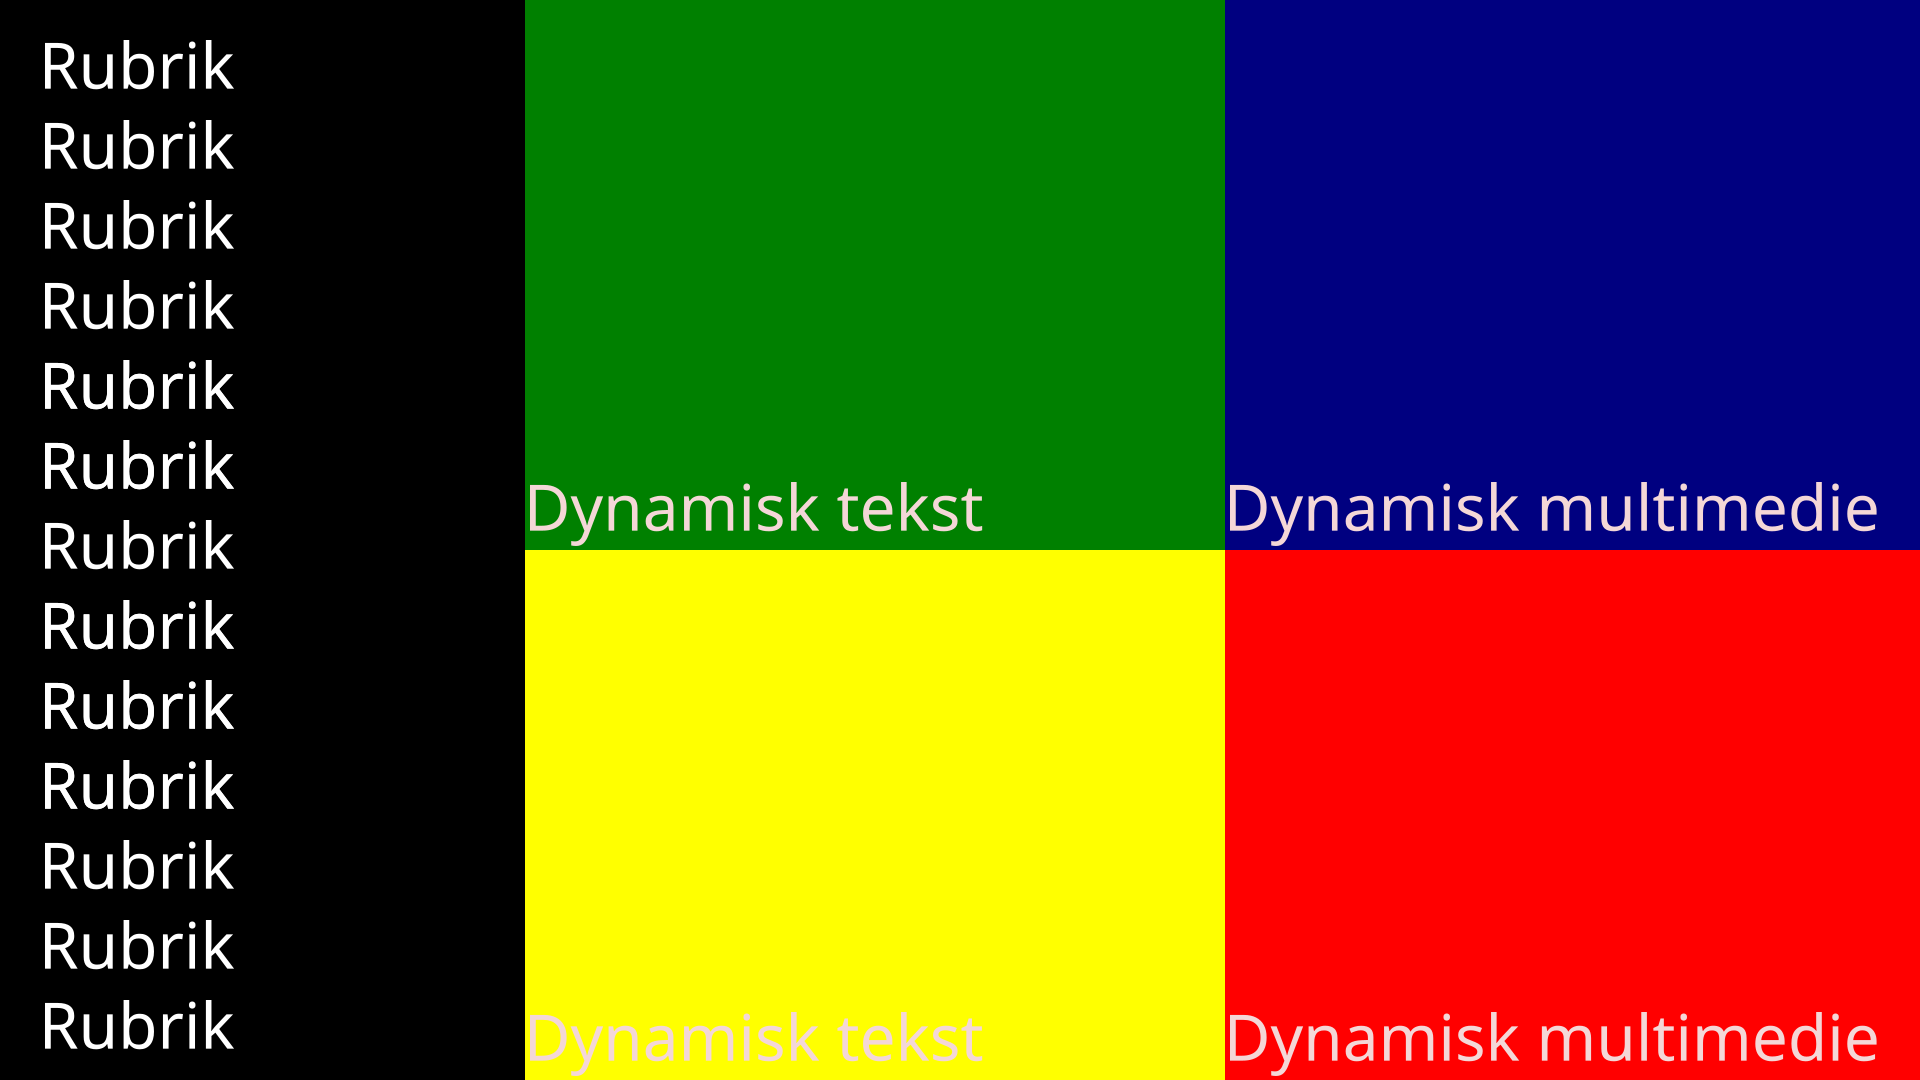
\includegraphics[width=\textwidth]{assets/section_6/Illustration-dynamic-routes.png}}
    \caption{Viser illustration af routes-systemet}
    \label{fig:routes}
\end{figure}

I det her tilfælde, laves datakald til en JSON-fil\footnote{JSON (JavaScript Object Notation) filer er et letvægts- læsbart filformat, som bruges til at organisere--strukturere information.}. Denne svarer i samme format, som en database ville, hvorfor dette er anvendt til at demonstrere datahåndteringsfunktionalitet uden at en reel database er nødvendig. I kapitlet \ref{sec:produktionsforberedelse} kan der læses mere om en eventuel implementering af en database.

\subsubsection{E-beregner}
E-beregneren er en simpel beregner, der har til formål at informere brugeren om, hvor stort deres kalorieindstag skal være ud fra nogle data. Denne tager højde for BMR, basalmetabolisme, som udgør ca 70\% af totalenergiforbruget og PA, fysisk aktivitet, som udgør ca. 20\% men ikke DIT, diætinduceret varmedannelse, som udgør 10\%\cite{EE-artikel}.

\paragraph{Matematikken}
Til formålet anvendes basalmetabolisme, som beskriver et varmblodet dyrs stofskifte.\cite{BMR-artikel} Her tages udgangspunkt i menneskets basalmetabolisme. Til dette formål anvendes Harris-Benedict-formlen, som er blevet revideret af Mifflin og St. Jeor i 1990\cite{Harris-Benedict-formel}, der ser således ud:

For mænd:
\begin{equation*}
    \text{BMR} \left[\dfrac{\text{kcal}}{\text{dag}}\right] = (10 \cdot \text{vægt [kg]}) + (6,25 \cdot \text{højde [cm]}) - (5 \cdot \text{alder [år]}) + 5
\end{equation*}

For kvinder:
\begin{equation*}
    \text{BMR} \left[\dfrac{\text{kcal}}{\text{dag}}\right] = (10 \cdot \text{vægt [kg]}) + (6,25 \cdot \text{højde [cm]}) - (5 \cdot \text{alder [år]}) - 161
\end{equation*}

Forskellen i formlen, skyldes mænd har en lidt højere basalmetabolisme end kvinder.

For at estimere det resterende kalorieforbrug, multipliceres BMR med en konstant, som afhænger af en persons fysiske aktivitet. Tallene er fundet fra en beregner på nettet med lignende funktionalitet \cite{OMNI-calc}:
\begin{table}[H]
    \centering
    \begin{tabular}{|c|c|}
        \hline
        \textbf{Aktivitet} & \textbf{Konstant} \\
        \hline
        Sedentær & 1,2 \\
        Lidt eller ingen aktivitet & 1,4 \\
        Let aktivitet 1-2 gange om ugen & 1,6 \\
        Moderat Aktivitet 2-3 gange om ugen & 1,75 \\
        Hård aktivitet 3-5 gange om ugen & 2 \\
        Fysisk job eller hård daglig aktivitet & 2,4 \\
        \hline
    \end{tabular}
\end{table}

ergo:
\begin{equation*}
    \text{Beregnet kalorieindtag} = \text{BMR} \cdot \text{aktivitetskonstant}
\end{equation*}

\paragraph{Implementering}
Forneden er kodeimplementeringen af formlen: 
\begin{mdframed}[backgroundcolor=blue!5]
\begin{minted}[
    framesep=2mm,
    baselinestretch=1.2,
    fontsize=\footnotesize,
    breaklines=true,
    breakanywhere=true,
]{typescript}
let bmr = 0;
if (currentEntry.koen.toLowerCase() === "mand") {
    // Harris-Benedict equation Men
    bmr = (10 * parseFloat(currentEntry.vaegt)) 
          + (6.25 * parseFloat(currentEntry.hoejde)) 
          - (5 * parseFloat(currentEntry.alder)) + 5;
} else if (currentEntry.koen.toLowerCase() === "kvinde") {
    // Harris-Benedict equation women
    bmr = (10 * parseFloat(currentEntry.vaegt)) 
          + (6.25 * parseFloat(currentEntry.hoejde)) 
          - (5 * parseFloat(currentEntry.alder)) - 161;
}
const maintenanceCalories = Math.ceil((bmr * parseFloat(currentEntry.aktivitetsniveau)));
const g_oksekoed = maintenanceCalories / 2.5;
\end{minted}
\end{mdframed}
\footnotesize\texttt{Kilde: app/(tabs)/e-beregner/e-beregner.tsx, linje 42-51}

Brugeren indtaster divere værdier, herunder brugerens alder, vægt, højde, køn, aktivitesniveau og navn, i inputfelter, hvorefter disse kan tilgås i backenden\footnote{>>the part of a computer system or application that is not directly accessed by the user, typically responsible for storing and manipulating data.<< - Oxford Languages}. Først tjekker koden, om hvorvidt brugeren er en mand eller kvinde, hvorefter den anvender enten den mandlige eller kvindelige Harris-Benedict-formel. Alle ledene i formlen er ens, på nær det sidste led, som enten tillæger 5 kalorier for mænd og trækker 161 kalorier for kvinder. Selve køn-variablet omdannes til småt, for at sikre, at der ikke kommer nogle fejl i koden, også selvom brugeren kun kan vælge mellem to prædefinerede værdier, altså en form for intern fejlsikring.

Ellers tages vægten, som multipliceres med 10, højden med 6.25 og 5 for alderen. Disse værdier er kun de nuværende indtastede værdier, idet e-beregneren har multipersonfunktionalitet, hvilket vil sige, at værdierne låses, når selve beregningen er gennemført, hvorefter nye værdier kan indtastes, og derved oprettes en ny profil (beregning). Desuden eksemplficerer programmet det daglige kaloriebehovet i divese hverdagsgoder, i det her tilfælde, gram oksekød. Dette gøres ved at dividere det daglige kaloriebehov med 2,5 kalorier pr. gram oksekød, som er det gennemsnitlige energiindhold i oksekød.

Dette er en simplifikation af den oprindelige vision for programmet, som skulle have kommet med forslag til retter og måltider, alt efter brugerens behov. Læs mere om det i kapitlet \ref{sec:post_scriptum_om_vision}

\subsubsection{Afgrødeberegner}
Afgrødeberegneren er en simpel beregner, der beregner, hvor meget såsæd og areal, der skal til for at opnå en angiven mængde meludbytte. Beregningerne og slutresultatet er blevet gennemgået af Hortonom Morten Jensen.

\paragraph{Matematikken}

Arealfunktion:
\begin{flalign*}
    & \mathrm{\text{meludbytte [input]} = \text{Såareal [output]} \cdot \dfrac{kornudbytte}{\text{Såareal}} \cdot \dfrac{meludbytte}{kornudbytte}}\\
    & \mathrm{\iff \text{Såareal [output]} = \dfrac{\text{meludbytte [input]}}{\left(\dfrac{kornudbytte}{\text{Såareal}} \cdot \dfrac{meludbytte}{kornudbytte}\right)}}
\end{flalign*}

Sædfunktion:
\begin{flalign*}
    & \mathrm{\text{meludbytte [input]} = \dfrac{meludbytte}{kornudbytte} \cdot \dfrac{kornudbytte}{\text{sæd [output]}}} \\
    & \mathrm{\iff \text{meludbytte [input]} \cdot \text{sæd [output]} = \dfrac{meludbytte}{kornudbytte} \cdot kornudbytte}\\
    & \mathrm{\iff \text{sæd [output]} = \dfrac{meludbytte}{kornudbytte} \cdot \dfrac{kornudbytte}{meludbytte [input]}}
\end{flalign*}

\paragraph{Implementering heraf} Forneden er kodeimplementeringen af formlerne:
\begin{mdframed}[backgroundcolor=blue!5]
\begin{minted}[
    framesep=2mm,
    baselinestretch=1.2,
    fontsize=\footnotesize,
    breaklines=true,
    breakanywhere=true,
]{typescript}
const froe_pr_m2 = 300; 
const korn_pr_m2 = 0.5; 
const mel_udbytte = 0.75;

const onsket_mel = parseFloat(currentEntry.mel);
const nodvendigt_korn = onsket_mel / mel_udbytte;
const nodvendigt_areal = nodvendigt_korn / korn_pr_m2;

[...]
const antal_froe = (nodvendigt_areal * froe_pr_m2) / 40;

\end{minted}
\end{mdframed}
\footnotesize\texttt{Kilde: app/(tabs)/afgrøde-beregner/afgrøde-beregner.tsx, linje 36-47}

Brugeren indtaster meludbyttet i et inputfelt og trykker beregn, hvorefter en funktion af meludbytteinputet (onsket\_mel-konstanten) køres, som beregner den nødvendige mængde hvedesæd og arealallokeringen hertil for at opnå den ønskede mængde malet korn.

Udover at rendere resultatet heraf, så illustreres arealet ved hjælp af en kvadrat, hvis siderlængder er tilsvarende kvadratroden af det givne areal. Gitterlinjernes kvadrater svarer cirka til en kvadratmeter, hvorfor brugeren kan forstå, hvor stort arealet er. Dette er en vigtighed, da markers størrelse hurtigt kan bliver uoverskuelige, hvis de ikke holdes i perspektiv.

Fornede ses den visualisering af arealet, som koden laver:

\begin{figure}[H]
    \centering
    \fbox{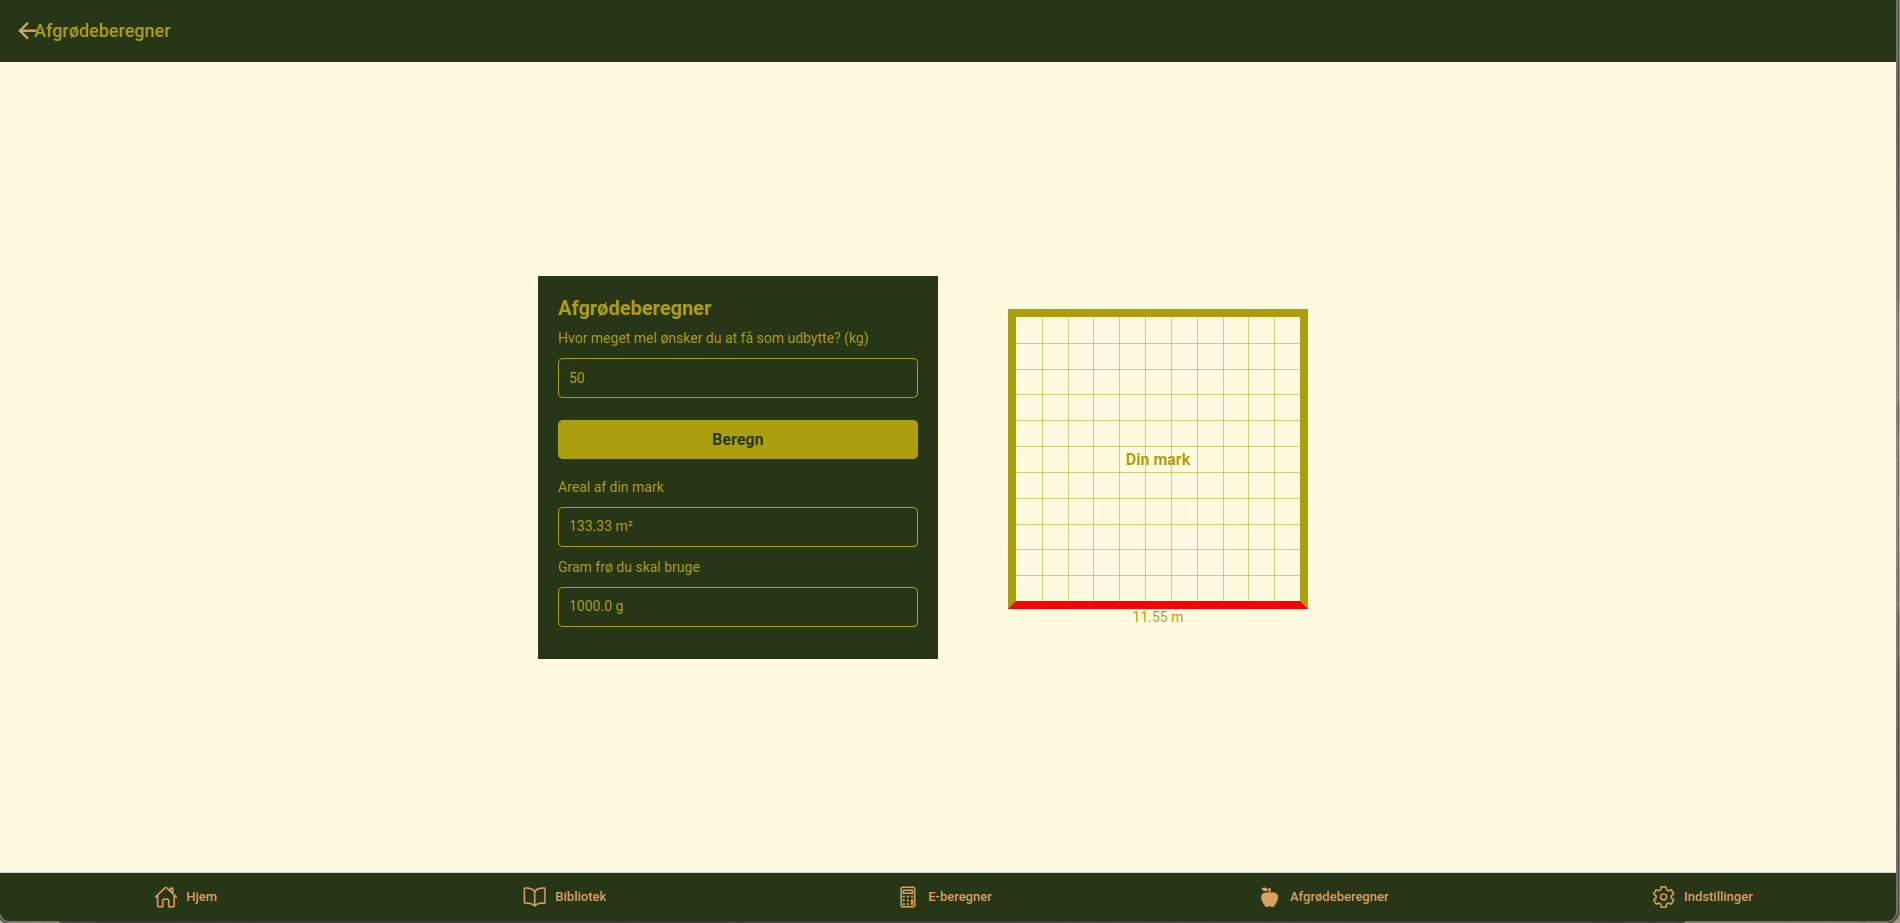
\includegraphics[width=\textwidth]{assets/section_6/arealberegner.png}}
    \caption{Viser visualiseringen af arealallokeringen, programmet laver.}
    \label{fig:arealberegner}
\end{figure}

\subsubsection{Indstillinger}

\paragraph{Forklaring} Indstillinger-siden er lavet, således at produkteretkriteriet omkring tilgænhelighed opfyldes. Det gøres ved, at der er en to switches\footnote{>>Switch<< er en visualisering af en sandhedsværdi, som enten er sand eller falsk, \break altså et binært 1 eller 0, en fysisk manifestation heraf kunne være en vippekontakt.}:
\begin{enumerate}
    \item En dysleksi-switch, der styrer om brugeren vil have en dysleksi-venlig skrifttype. Dysleksi-fonten, >>Open Dyslexic<<, er udviklet med videnskabelige undersøgelser om læsbarheden af tekst med henblik på at forbedre læsbarheden for dyslektikere, i minde\cite{OpenDyslexic}. Herfor er den selvsagt valgt. 
    \item en farveblindheds-switch, der styrer om alle elementer skal renderes farverigt eller sort-hvidt. Sort-hvid-paletten er valgt, da alle farveblinde vil kunne afkode elementer med disse nuancer, selv folk, der lider af monokromatisk farveblindhed\cite{colourblindness_awareness}.
\end{enumerate}

\paragraph{Implementering heraf}
\subparagraph{Dysleksi-switch} Forneden ses koden, der modtager input fra dysleksi-switchen og anvender dette til at indstille skrifttypen. Denne import sker i præamblen til en hvilkensomhelst fil, der indeholder tekst, som skal vises til brugeren:
\begin{mdframed}[backgroundcolor=blue!5]
\begin{minted}[
    framesep=2mm,
    baselinestretch=1.2,
    fontsize=\footnotesize,
    breaklines=true,
    breakanywhere=true,
]{typescript}
import { useFont } from "@/components/fontContext";
const { dyslexiaMode } = useFont();
\end{minted}
\end{mdframed}
\footnotesize\texttt{Kilde: Præamblen\footnote{>>Præamblen<< er det første kode, der køres. Heri kan metainformation angives om koden, fx titel, forfatter, dato, version, etc., men også kodningsrelevante elementer såsom importeringen af andre filer, konstanter, elementer, biblioteker, etc, som anvendes generelt eller senere i koden. Således indstilles "kodemiljøet" heri.} til en hvilkensomhelst fil, der indeholder tekst.}

Her ses teksten, hvori de importede >>themes<< (temaer) er anvendt i dennes style-værdi. Dette går igen igenem hele koden:
\begin{mdframed}[backgroundcolor=blue!5]
\begin{minted}[
    framesep=2mm,
    baselinestretch=1.2,
    fontsize=\footnotesize,
    breaklines=true,
    breakanywhere=true,
]{typescript}
{ fontFamily: dyslexiaMode ? 'open-dyslexic' : 'System' }
\end{minted}
\end{mdframed}
\footnotesize\texttt{Kilde: hvilkensomhelst teksts >>style<<-værdi.}

\subparagraph{Farveblindheds-switch} Forneden ses koden, der modtager input fra farveblindheds-switchen og anvender dette til at ændre farvepaletten:
\begin{mdframed}[backgroundcolor=blue!5]
\begin{minted}[
    framesep=2mm,
    baselinestretch=1.2,
    fontsize=\footnotesize,
    breaklines=true,
    breakanywhere=true,
]{typescript}
import { useTheme } from "@/components/themeContext";
import { normalTheme, colorBlindTheme } from "@/constants/themes";

const currentTheme = theme === 'normal' ? colorBlindTheme:normalTheme;
const { theme } = useTheme();
{ backgroundColor: currentTheme.calculatorBackground }
\end{minted}
\end{mdframed}
\footnotesize\texttt{Kilde: en hvilkensomhelst fil, der anvender en form for farvepallete, altså vises til brugeren.}

Forneden ses koden, hvor farvepalleterne, som eksporteres er, afhængigt af, hvad værdi, switchen har. Læg mærke til, at de forskellige farvepaletter, normalTheme og colorBlindTheme som er defineret i to rækker\footnote{>>Række<< er en række af elementer, som har et navn og en værdi, her et navn og en farve.}:
\begin{mdframed}[backgroundcolor=blue!5]
\begin{minted}[
    framesep=2mm,
    baselinestretch=1.2,
    fontsize=\footnotesize,
    breaklines=true,
    breakanywhere=true,
]{typescript}
export const normalTheme = {
    background: "#222b00",
    headerColor: "#283618",
    arrowIconColor: "#dda15e",
    fontColor: "#ac9f0d",
    tabBarActiveTintColor: "#dda15e",
    tabBarInactiveTintColor: "#dda15e",
    bibLinkStyle: "#DDA15E",
    bibBackground: "#283618",
    grejLinkStyle: "#000",
    grejIconColor: "#dda15e",
    calculatorBackground: "#fefae0",
    redBlack: "black",
    blackRed: "red",
    calculatorButton: "#000",
    newBibBackground: "#fefae0",
    grejViAnbefaler: "#dda15e",
    afgrødeBeregnerButton: "#0000FF",
}

export const colorBlindTheme = {
    background: "#fff",
    headerColor: "#fff",
    arrowIconColor: "#000",
    fontColor: "#000",
    tabBarActiveTintColor: "#000",
    tabBarInactiveTintColor: "#000",
    bibLinkStyle: "#000",
    bibBackground: "#fff",
    grejLinkStyle: "#000",
    grejIconColor: "#fff",
    calculatorBackground: "#fff",
    redBlack: "red",
    blackRed: "black",
    calculatorButton: "#0000FF",
    newBibBackground: "#fff",
    grejViAnbefaler: "#000",
    afgrødeBeregnerButton: "#000",
}
\end{minted}
\end{mdframed}
\footnotesize\texttt{Kilde: constants/themes.ts, linje 1-39}

Andre forslag til "indstillinger-siden" \space findes i post scriptummet omkring visionen for produktet\ref{sec:post_scriptum_om_vision}.